\chapter{Domain-adaptive neural networks improve supervised machine learning based on simulated population genetic data}

\textit{Content of this chapter was previously uploaded to bioRxiv (2023) under the title ``Domain-adaptive neural networks improve supervised machine learning based on simulated population genetic data" by Ziyi Mo and Adam Siepel. The manuscript was published in PLoS Genetics (2023) under the same title.}

\section{Abstract}
Investigators have recently introduced powerful methods for population genetic inference that rely on supervised machine learning from simulated data. Despite their performance advantages, these methods can fail when the simulated training data does not adequately resemble data from the real world. Here, we show that this “simulation mis-specification” problem can be framed as a “domain adaptation” problem, where a model learned from one data distribution is applied to a dataset drawn from a different distribution. By applying an established domain-adaptation technique based on \iac{GRL}, originally introduced for image classification, we show that the effects of simulation mis-specification can be substantially mitigated. We focus our analysis on two state-of-the-art deep-learning population genetic methods—\ac{SIA}, which infers positive selection from features of the \acf{ARG}, and ReLERNN, which infers recombination rates from genotype matrices. In the case of \ac{SIA}, the domain adaptive framework also compensates for \ac{ARG} inference error. Using the \ac{dadaSIA} model, we estimate improved selection coefficients at selected loci in the 1000 Genomes CEU population. We anticipate that domain adaptation will prove to be widely applicable in the growing use of supervised machine learning in population genetics.

\section{Introduction}
Advances in genome sequencing have allowed population genetic analyses to be applied to many thousands of individual genome sequences (\cite{auton_global_2015,sudlow_uk_2015,karczewski_mutational_2020}). Given adequately rigorous and scalable computational tools for analysis, these rich catalogs of genetic variation provide opportunities for addressing many important questions in areas such as human evolution, plant genetics, and the ecology of non-model organisms. Deep-learning methods, already well-established in other application areas (\cite{lecun_deep_2015}), have proven to be good matches for these analytical tasks and have recently been successfully applied to many problems in population genetics (\cite{sheehan_deep_2016,kern_diploshic_2018,schrider_supervised_2018,flagel_unreasonable_2019,torada_imagene_2019,adrion_predicting_2020,caldas_inference_2022,hejase_deep-learning_2022,korfmann_deep_2023,huang_harnessing_2023}).

The key to the success of deep learning in population genetics has been the use of large amounts of simulated data for training. Under simplifying, yet largely realistic, assumptions, evolution plays by relatively straightforward rules. By exploiting these rules and advances in computing power, a new generation of computational simulators has made it possible to efficiently produce large quantities of perfectly labeled synthetic data across a wide range of evolutionary scenarios (\cite{haller_tree-sequence_2019,haller_slim_2019,baumdicker_efficient_2022}). At the same time, programming libraries such as stdpopsim have made these simulators accessible to a broad community of researchers while improving the reproducibility of simulation workflows (\cite{adrion_community-maintained_2020,lauterbur_expanding_2022}). The facility of generating synthetic training data serves as the foundation of the new simulate-and-train paradigm of supervised machine learning for population genetics inference (Fig. \ref{fig:DA-F1}A; \cite{schrider_supervised_2018,korfmann_deep_2023,huang_harnessing_2023}).

\begin{figure}[h]
    \centering
    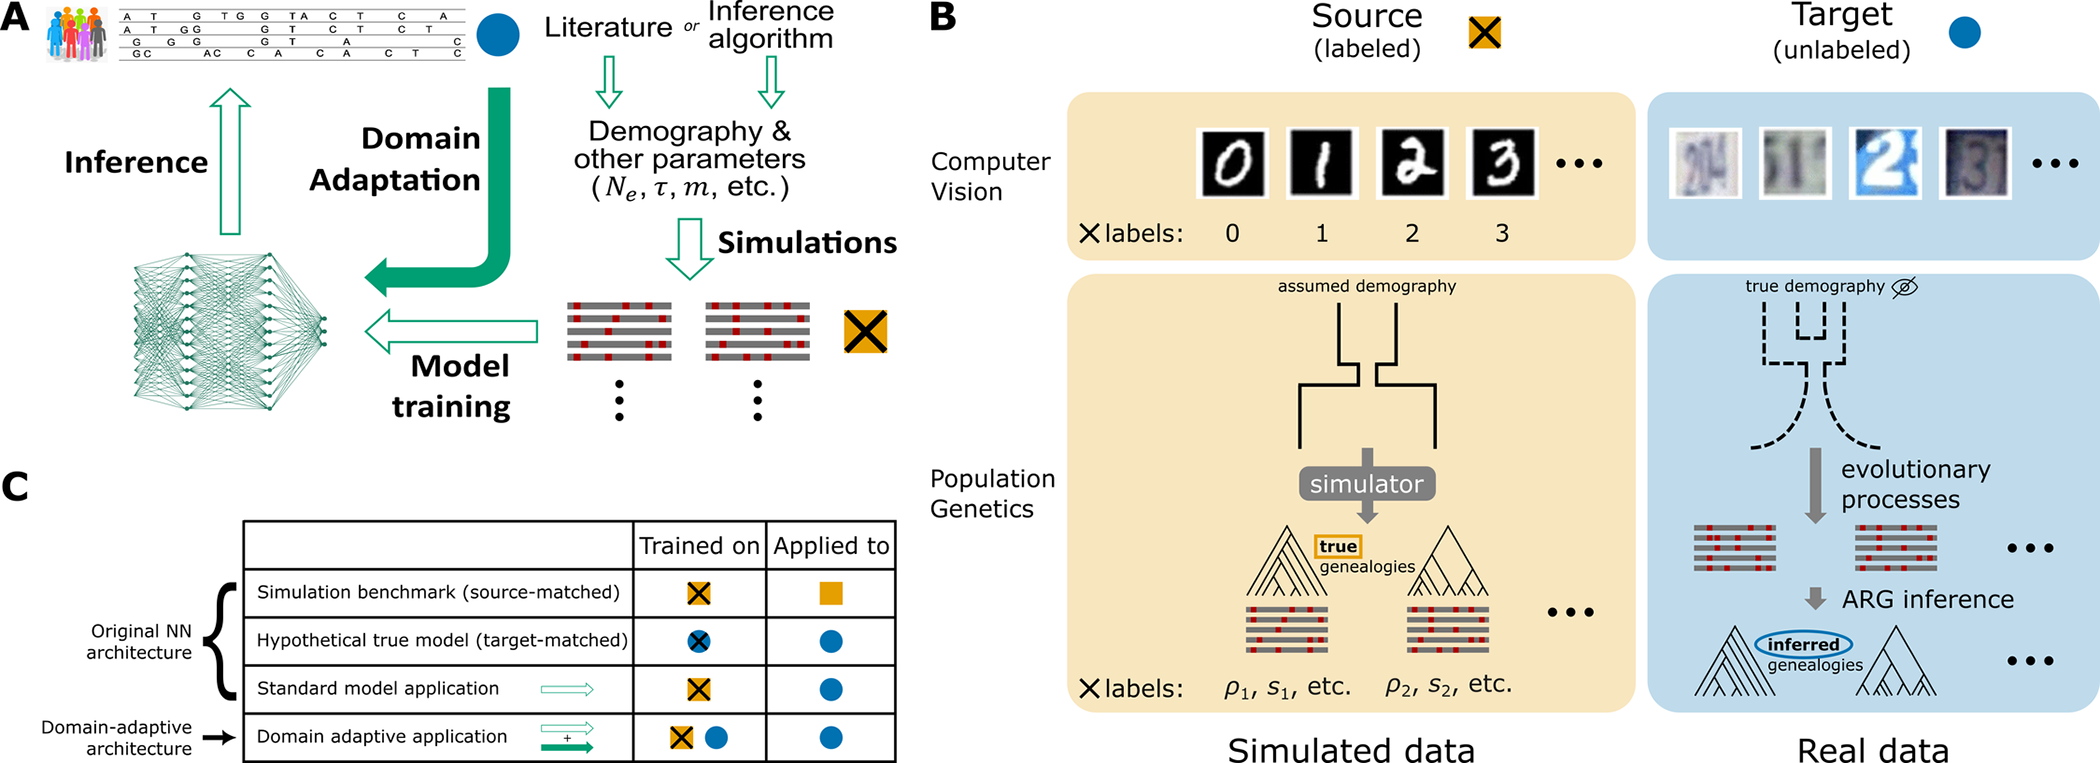
\includegraphics[width=\textwidth]{DA_figs/DA_F1.PNG}
    \caption[Unsupervised domain adaptation in the context of population genetic inference.]{\textbf{Unsupervised domain adaptation in the context of population genetic inference.} \textbf{A)} A high-level overview of the supervised machine-learning approach for population genetic inference and how domain adaptation fits into the paradigm. \textbf{B)} Example formulations of the unsupervised domain adaptation problem with application to computer vision and population genetics. Note that in the specific case of \ac{SIA}, which uses features of the \ac{ARG}, the source domain data always consist of true genealogies generated in simulations, whereas the target domain data always consist of inferred genealogies reconstructed from observed sequence data. \textbf{C)} Four benchmarking scenarios considered in this study. The original model was both trained and tested on source domain data (simulation benchmark), both trained and tested on target domain data (hypothetical true model), or trained on source domain data but applied to target domain data (standard model application). These three cases contextualize the performance of the domain-adaptive model (see \nameref{DA-methods} for details). Gold squares represent source domain data, blue circles represent target domain data and crosses ($\mathbf{\times}$) represent labels.}
    \label{fig:DA-F1}
\end{figure}

At the same time, this paradigm is highly dependent on well-specified models for simulation (\cite{korfmann_deep_2023}). If the simulation assumptions do not match the underlying generative process of the real data -- that is, in the presence of \textit{simulation mis-specification} -- the trained deep-learning model may reflect the biases in the simulated data and perform poorly on real data. Indeed, previous studies have shown that, despite being robust to mild to moderate levels of mis-specification, performance inevitably degrades when the mismatch becomes severe (\cite{adrion_predicting_2020,hejase_deep-learning_2022}).

In a typical workflow, key simulation parameters such as the mutation rate, recombination rate, and parameters of the demographic model are either estimated from the data or obtained from the literature (Fig. \ref{fig:DA-F1}A; \cite{adrion_community-maintained_2020,lauterbur_expanding_2022}). Sometimes these parameters are allowed to vary during simulation, and sometimes investigators evaluate the sensitivity of predictions to departures from the assumed range, but there is typically no way to ensure that the ranges considered are adequately large. Moreover, these benchmarks do not usually account for under-parameterization of the demographic model. Particularly in the case of non-model organisms, the quality of the estimates can be further limited by the availability of data. Overall, some degree of mis-specification in the simulated training data is impossible to avoid.

One way to mitigate the effects of simulation mis-specification would be to engineer a simulator to force the simulated data to be compatible with real data. For example, one could simulate from an overdispersed distribution of parameters followed by a rejection sampling step (based on summary statistics) as in \acf{ABC} methods, or one could use a \ac{GAN} (\cite{wang_automatic_2021}) to mimic the real data. These methods tend to be costly, however. For example, \ac{ABC} methods scale poorly with the dimensionality of the parameter space, and \acp{GAN} are notoriously hard to train.

Here we consider the alternative approach of adopting a deep-learning model that is explicitly designed to account for and mitigate the mismatch between simulated and real data (Fig. \ref{fig:DA-F1}A). A standard machine learning model aims to make accurate predictions on data following the same probability distribution as the training instances. In contrast, the task of building well-performing models for a target dataset that has a \textit{different} distribution from the training dataset is termed “domain adaptation” in the machine-learning literature (\cite{csurka_comprehensive_2017,wilson_survey_2020}). A typical setting of interest for domain adaptation is image classification (Fig. \ref{fig:DA-F1}B). For example, suppose a digit-recognition model is needed for the Street View House Numbers (SVHN) dataset (the “target domain”), but abundant labeled training data is only available from the MNIST dataset of handwritten digits (the “source domain”). In this case, a method needs to train on one dataset and perform well on another, despite systematic differences between the two data distributions.

Various strategies for domain adaptation have been introduced. Prior to the advent of deep learning, early methods focused on reweighting training instances according to their likelihoods of being a source or target example (\cite{shimodaira_improving_2000,dai_boosting_2007}) or explicitly manipulating a feature space through augmentation (\cite{daume_iii_frustratingly_2009}), alignment (\cite{fernando_unsupervised_2013,sun_return_2016}) or transformation (\cite{pan_domain_2011}). Recently, specialized neural network architectures have been developed for deep domain adaptation. Most model architectures of this kind share the common goal of learning a “domain-invariant” representation of the data through a feature extractor neural network, for example, by minimizing domain divergence (\cite{rozantsev_beyond_2019}), by adversarial training (\cite{ganin_unsupervised_2014,liu_coupled_2016}) or through an auxiliary reconstruction task (\cite{ghifary_deep_2016}). Domain adaptation so far has been most widely applied in the fields of computer vision (e.g., using stock photos for semantic segmentation of real photos) and natural language processing (e.g., using Amazon product reviews for sentiment analysis of movies and TV shows) where large, heterogeneous datasets are common but producing labeled training examples can be labor intensive (\cite{wilson_survey_2020}). More recently, deep domain adaptation has been used in regulatory genomics to enable cross-species transcription-factor-binding-site prediction (\cite{cochran_domain-adaptive_2022}).

In this work, we reframe the simulation mis-specification problem in population genetics as an unsupervised domain adaptation problem -- unsupervised in the sense that data from the target domain is not labeled (Fig. \ref{fig:DA-F1}B). In particular, we use population-genetic simulations to obtain large amounts of perfectly labeled training data in the source domain. We then seek to apply the trained model to unlabeled real data in the target domain. We use domain adaptation techniques to explicitly account for the mismatch between these two domains when training the model.

To demonstrate the feasibility of this approach, we incorporated a domain-adaptive neural network architecture into two published deep learning models for population genetic inference: 1) SIA (\cite{hejase_deep-learning_2022}), which identifies selective sweeps based on the \acf{ARG}, and 2) ReLERNN (\cite{adrion_predicting_2020}), which infers recombination rates from raw genotypic data. Through extensive simulation studies, we demonstrated that the domain adaptive versions of the models significantly outperformed the standard versions under realistic scenarios of simulation mis-specification. Our domain-adaptive framework for utilizing mis-specified synthetic data for supervised learning opens the door to many more applications in population genetics.

\section{Results}

\subsection{Experimental design}
We created domain-adaptive versions of the \ac{SIA} and ReLERNN models, each of which employed a \acf{GRL} (\cite{ganin_unsupervised_2014}) (Fig. \ref{fig:DA-F2}A\&B). As noted, the goal of domain adaptation is to establish a “domain-invariant” representation of the data (Fig. \ref{fig:DA-F1}A). Our neural networks consist of two major components: the original networks (“feature extractor” in green and “label predictor” in blue in Fig. \ref{fig:DA-F2}A\&B), which are applied only to labeled examples from the “source” (simulated) domain; and alternative branches (“domain classifier” in yellow in Fig. \ref{fig:DA-F2}A\&B), which use the same feature-extraction portions of the first networks but have the distinct goal of distinguishing data from the “source” (simulated) and “target” (real) domains (they are applied to both). When the neural network is trained by back-propagation, the \ac{GRL} reverses the sign of the gradient for the feature extractor with respect to the domain-classifier loss. By doing so, the \ac{GRL} systematically undermines this secondary goal of distinguishing the two domains (Fig. \ref{fig:DA-F2}, see \nameref{DA-methods} for details), and therefore promotes domain invariance in feature extraction.

\begin{figure}
    \centering
    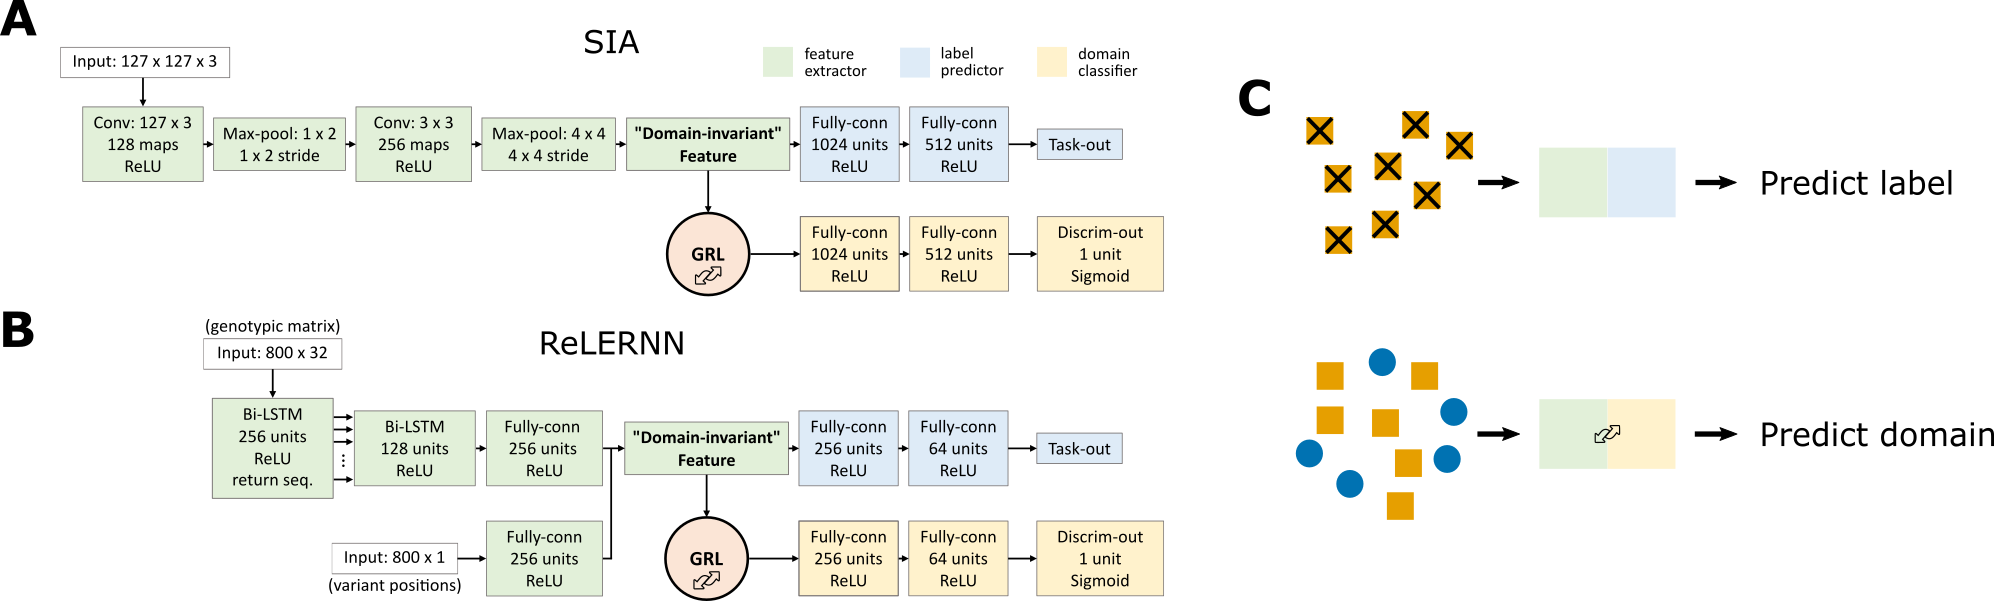
\includegraphics[width=\textwidth]{DA_figs/DA_F2.PNG}
    \caption[Neural network architecture for domain adaptation.]{\textbf{Neural network architecture for domain adaptation.} The model architectures incorporating \acfp{GRL} for \textbf{A)} \ac{SIA} and \textbf{B)} ReLERNN. The feature extractor of \ac{SIA} contains $1.49 \times 10^5$ trainable parameters, whereas the label predictor and domain classifier contains $1.22 \times 10^8$ each. The feature extractor of ReLERNN contains $1.52 \times 10^6$ trainable parameters, whereas the label predictor and domain classifier contains $1.49 \times 10^5$ each. Note that the total number of trainable parameters includes those in batch normalization layers. \textbf{C)} When training the networks, each minibatch of training data consists of two components: (1) labeled data from the source domain fed through the feature extractor and the label predictor; and (2) a mixture of unlabeled data from both the source and target domains fed through the feature extractor and the domain classifier. The first component trains the model to perform its designated task. However, the \ac{GRL} inverts the loss function for the second component, discouraging the model from differentiating the two domains and leading to the extraction of “domain-invariant” features.}
    \label{fig:DA-F2}
\end{figure}

We designed two sets of benchmark experiments to assess the performance of the domain-adaptive models relative to the standard models. In both cases, we tested the methods using “real” data in the target domain that was actually generated by simulation, but included features not considered by the simpler simulator used for the source domain. In the first set of experiments, background selection was present in the target domain but not the source domain. In the second set of experiments, the demographic model used for the source-domain simulations was estimated from “real” data generated under a more complex demographic model and was therefore somewhat mis-specified (as detailed below). Below we refer to these as the “background selection” and “demography mis-specification” experiments.

\subsection{Performance of domain-adaptive \ac{SIA} model}
We compared the performance of the \acf{dadaSIA} model to that of the standard \ac{SIA} model on held-out “real” data, considering both a classification (distinguishing selective sweeps from neutrality) and a regression (inferring selection coefficients) task. In all cases, we focused on a comparison of the domain-adaptive model to the standard case where a model is simply trained on data from the source domain and then applied to the target domain (“standard model”; Fig. \ref{fig:DA-F1}C). Note that the version of \ac{SIA} used by both the domain-adaptive and standard models includes a variety of minor improvements that led to modest gains in performance over the previously published version (see \textit{Updates to genealogical features and deep learning architecture for the \ac{SIA} model} in \nameref{DA-methods} and Fig. \href{https://journals.plos.org/plosgenetics/article?id=10.1371/journal.pgen.1011032#sec018}{S1B\&C online}). The codebase of the original \ac{SIA} model has been updated accordingly.

For additional context, we also considered the two cases where the training and testing domains matched (“source-matched” or “target-matched”; Fig. \ref{fig:DA-F1}C)—although we note that these cases are not achievable with real data and provide only hypothetical upper bounds on performance. Notably, in the source-matched (or “simulation benchmark”) case, the standard model is both trained and tested with true genealogies from source-domain simulations. By contrast, in the target-matched (or “hypothetical true model”) case, the standard model is trained as if target-domain data with ground-truth selection coefficient labels were available. Since genealogies need to be inferred in the target domain (Fig. \ref{fig:DA-F1}B), the hypothetical true model is both trained and tested with inferred genealogies (see \textit{Setup of benchmarking experiments} in \nameref{DA-methods} for details).

As noted, we considered two types of mis-specification, background selection and demographic mis-specification. In the background selection experiments, the target domain experienced selection in a central “genic” region (following a \acsu{DFE} from \cite{boyko_assessing_2008}), leading to background selection in flanking regions. This genic region was omitted in the source domain. In the demographic mis-specification experiments, the demographic model for source-domain simulations was inferred from “real” data using G-PhoCS (\cite{gronau_bayesian_2011}). Both the real (target domain) and inferred (source domain) models assumed three populations with migration, but the inferred model was under-parameterized and its parameters differed substantially from the real model (Fig. \href{https://journals.plos.org/plosgenetics/article?id=10.1371/journal.pgen.1011032#sec018}{S1A online}) (see \nameref{DA-methods} for details).

In both the background selection and demography mis-specification experiments, and in both the classification and regression tasks, the domain-adaptive \ac{SIA} model substantially improved on the standard model (Fig. \ref{fig:DA-F3}). Indeed, in all cases, the domain-adaptive model (turquoise lines in Fig. \ref{fig:DA-F3}A\&C) nearly achieved the upper bound of the hypothetical true model (dashed gray lines) and clearly outperformed the standard model (gold lines), suggesting that domain adaptation had largely “rescued” \ac{SIA} from the effects of simulation mis-specification (see also Fig. \href{https://journals.plos.org/plosgenetics/article?id=10.1371/journal.pgen.1011032#sec018}{S2C\&D online}). The standard model performed particularly poorly on the regression task (Fig. \ref{fig:DA-F3}B\&D), but the domain-adaptive model achieved substantial improvements, reducing both the absolute error as well as the upward bias of the estimation (Fig. \href{https://journals.plos.org/plosgenetics/article?id=10.1371/journal.pgen.1011032#sec018}{S2C\&D online}).

\begin{figure}
    \centering
    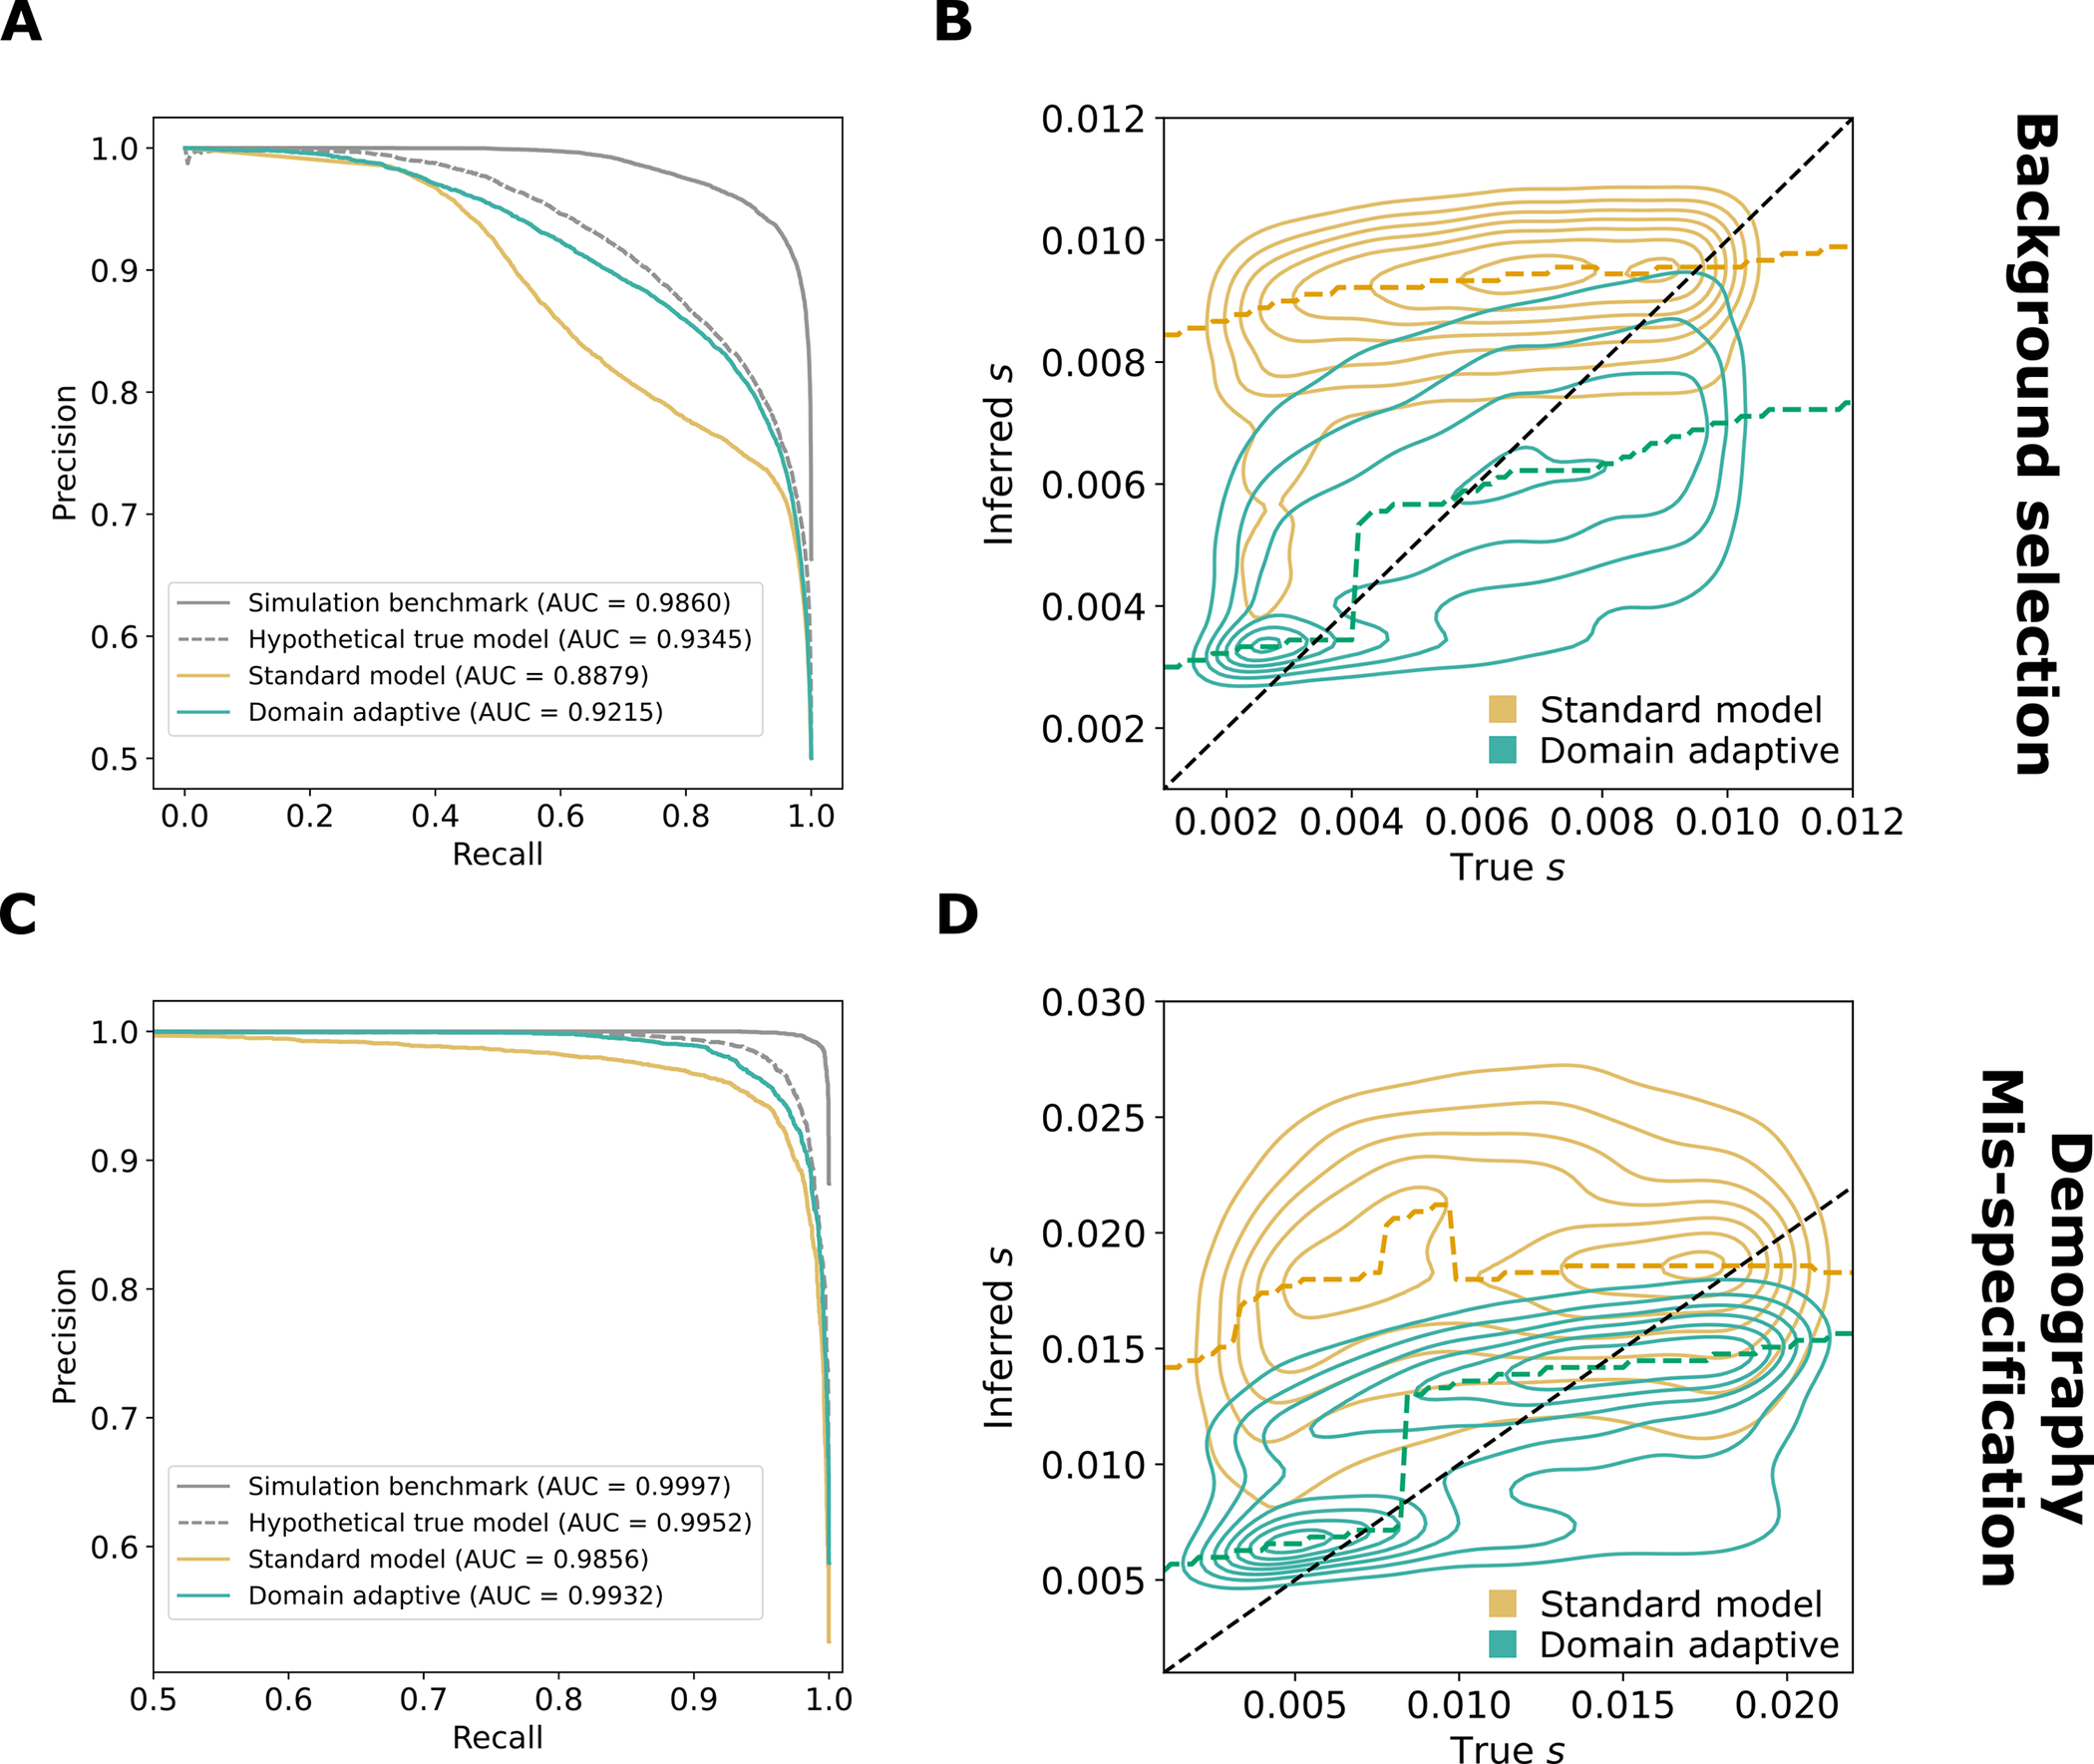
\includegraphics[width=\textwidth]{DA_figs/DA_F3.PNG}
    \caption[Performance of domain-adaptive \ac{SIA} models.]{\textbf{Performance of domain-adaptive \ac{SIA} models.} Results are shown from (\textbf{A}, \textbf{B}) the background-selection and (\textbf{C}, \textbf{D}) the demography-mis-specification experiments. (\textbf{A}, \textbf{C}) Precision-recall curves for sweep classification. (\textbf{B}, \textbf{D}) Contour plots summarizing true (horizontal axis) vs. inferred (vertical axis) selection coefficients ($s$) for the standard (gold) and domain adaptive (turquoise) models as evaluated on the held-out test dataset. The ridge along the horizontal axis of each contour is traced by a dashed line, representing the mode of the inferred value for each true value of $s$. Raw data underlying the contour plots are presented in Fig. \href{https://journals.plos.org/plosgenetics/article?id=10.1371/journal.pgen.1011032\#sec018}{S2 online}. See Fig. \ref{fig:DA-F1}C for definition of the model labels.}
    % https://tex.stackexchange.com/questions/366909/and-other-characters-in-a-url
    \label{fig:DA-F3}
\end{figure}

The comparisons with the simulation benchmark and hypothetical true model were also informative in other ways. Notice that performance in the simulation benchmark case was considerably better than that in all other cases, including the hypothetical true model. For \ac{SIA} in particular, the \ac{ARG} is “known” (fixed in simulation) in the source domain, whereas in the target domain it must be inferred (Fig. \ref{fig:DA-F1}B). Thus, the difference between the simulation benchmark (source-matched) and hypothetical true model (target-matched) cases represents a rough measure of the importance of \ac{ARG} inference error (see \nameref{DA-discussion}). In addition, note that in many studies, benchmarking of population-genetic models is performed using the same, or similar, simulations as those used for training, as with our hypothetical true model. Thus, the difference between the hypothetical true model and the standard model is representative of the degree to which benchmarks of this kind may be overly optimistic about performance, depending on the degree to which the simulations are mis-specified.

We further investigated the effect of imbalanced training data from the target domain on the performance of the domain-adaptive model in the context of sweep classification. Despite the ability to simulate perfectly class-balanced labeled data in the source domain, in practice we have no control over whether real data are balanced. Using simulations for the background selection mis-specification experiments, we tested the performance of the domain-adaptive \ac{SIA} model classifying sweeps when trained with unlabeled “real” data under different proportions of sweep vs. neutral examples. While a balanced dataset yielded the best performance, significantly skewed datasets (20\% or 80\% sweep examples) still provided the domain-adaptive model with reasonable improvement upon the standard model (Fig. \href{https://journals.plos.org/plosgenetics/article?id=10.1371/journal.pgen.1011032\#sec018}{S3A\&B online}). The exception appeared to be when the target domain data consisted entirely of sweep examples (100\% sweep). Although highly unrealistic, this scenario demonstrates that the domain-adaptive model can underperform the standard model when the target domain data follow a radically different distribution.

Another type of imbalance arises if only a limited amount of target domain data is available to train the domain-adaptive model. Using the same set of simulations for the background selection mis-specification experiments, we tested the performance of the domain-adaptive \ac{SIA} model when trained with less target domain data. With the target domain data at only 10\% of the source domain data (source:target ratio = 10:1), the model suffered a noticeable drop in performance yet still maintained a clear advantage over the standard model (Fig. \href{https://journals.plos.org/plosgenetics/article?id=10.1371/journal.pgen.1011032\#sec018}{S3C-E online}). We did not examine the case where there is more target domain than source domain data, since one could always simulate additional source domain data to match the size of the target domain. In summary, our experiments suggest that domain adaptation can accommodate reduced or imbalanced data for the target domain but there is a cost in performance if the reduction or imbalance is extreme.

\subsection{Performance of domain-adaptive ReLERNN model}
We performed a parallel set of experiments with a domain-adaptive version of ReLERNN. In this case, the background selection experiment was essentially the same as for \ac{SIA}, but we used a simpler design for the demography mis-specification experiment, following \cite{adrion_predicting_2020}. Briefly, the “real” (target domain) data was generated according to the out-of-Africa European demographic model estimated by \cite{tennessen_evolution_2012}. By contrast, the simulated data for the source domain simply assumed a constant-sized panmictic population at equilibrium with $N_e=\frac{\hat{\theta}_W}{4\mu}$, where  $\hat{\theta}_W$ is the Watterson estimator obtained from the “real” data (see \nameref{DA-methods} for details).

Similar to our results for \ac{SIA}, the domain-adaptive ReLERNN model both reduced the \ac{MAE} and corrected for the downward bias in recombination-rate estimates compared to the standard model (Figs. \ref{fig:DA-F4} and \href{https://journals.plos.org/plosgenetics/article?id=10.1371/journal.pgen.1011032#sec018}{S6 online}). In the background-selection experiment, the standard ReLERNN model performed quite well (Figs. \ref{fig:DA-F4}A and \href{https://journals.plos.org/plosgenetics/article?id=10.1371/journal.pgen.1011032#sec018}{S6A online}, $\mathrm{MAE} = 5.60\times 10^{-9}$), but the domain-adaptive ReLERNN model nonetheless further reduced the MAE to $4.41\times 10^{-9}$ (Fig. \href{https://journals.plos.org/plosgenetics/article?id=10.1371/journal.pgen.1011032#sec018}{S6C online}, Welch’s $t$-test: $n = 25,000$, $t =31.0$, $p<10^{-208}$). The advantage of the domain-adaptive model was more apparent in the demography-mis-specification experiment (Figs. \ref{fig:DA-F4}B and \href{https://journals.plos.org/plosgenetics/article?id=10.1371/journal.pgen.1011032#sec018}{S6B online}), where it reduced the MAE from $8.06\times 10^{-9}$ to $5.45\times 10^{-9}$ (Fig. \href{https://journals.plos.org/plosgenetics/article?id=10.1371/journal.pgen.1011032#sec018}{S6D online}, Welch’s $t$-test, $n = 25,000$, $t = 72.4$, $p<10^{-323}$). Notably, our results for the standard model in the demography-mis-specification experiment were highly similar to those reported by \cite{adrion_predicting_2020}, including the approximate mean and range of the raw error (compare \href{https://academic.oup.com/view-large/figure/204168641/msaa038f4.tif}{Fig. 4A} from \cite{adrion_predicting_2020} and Fig. \href{https://journals.plos.org/plosgenetics/article?id=10.1371/journal.pgen.1011032#sec018}{S6D online}), as well as the downward bias.

\begin{figure}[h]
    \centering
    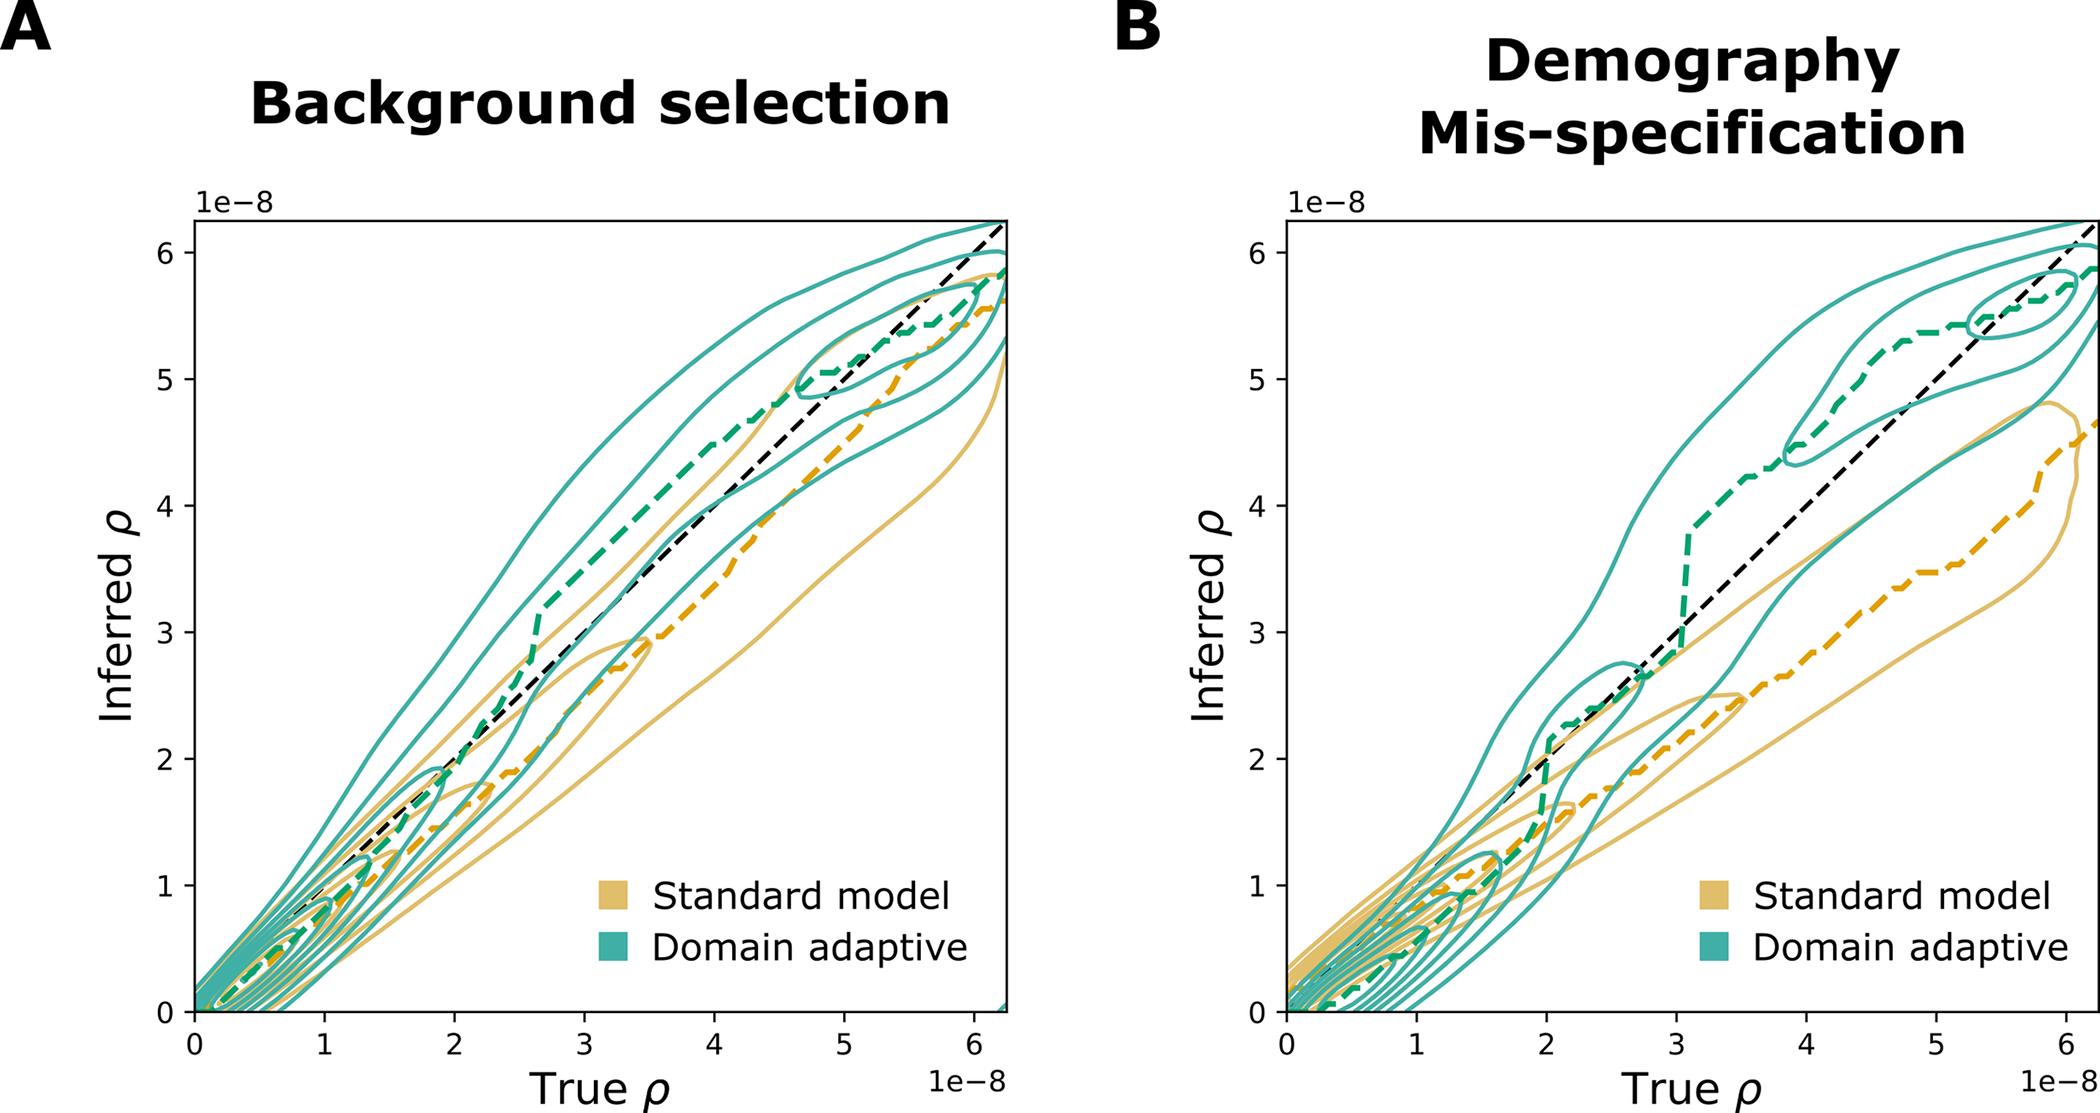
\includegraphics[width=\textwidth]{DA_figs/DA_F4.PNG}
    \caption[Performance of domain-adaptive ReLERNN models.]{\textbf{Performance of domain-adaptive ReLERNN models.} Results are shown from (\textbf{A}) the background-selection and (\textbf{B}) the demography-mis-specification experiments. Each contour plot summarizes true (horizontal axis) vs. inferred (vertical axis) recombination rates ($\rho$) for the standard (gold) and domain adaptive (turquoise) models as evaluated on the held-out test dataset. The ridge along the horizontal axis of each contour is traced by a dashed line, representing the mode of the inferred value for each true value of $\rho$. Raw data underlying the contour plots are presented in Fig. \href{https://journals.plos.org/plosgenetics/article?id=10.1371/journal.pgen.1011032\#sec018}{S6 online}.}
    \label{fig:DA-F4}
\end{figure}

Interestingly, \cite{adrion_predicting_2020} observed that ReLERNN was sometimes more strongly influenced by demographic mis-specification than unsupervised methods such as LDhelmet, even though it still performed better in terms of absolute error. The addition of domain adaptation appears to considerably mitigate this susceptibility to demographic mis-specification, making an excellent method even stronger.

\subsection{Efficacy of domain adaptation under various degrees of simulation mis-specification}
So far, we have examined scenarios of relatively modest simulation mis-specifica\\-tion, likely to be encountered in real applications. While domain adaptation appeared to be effective in these cases, we expect a limit to its capability when mis-specification is extreme. We therefore carried out a series of experiments to probe the performance of the \ac{dadaSIA} model under increasingly severe simulation mis-specification (Fig. \href{https://journals.plos.org/plosgenetics/article?id=10.1371/journal.pgen.1011032#sec018}{S4 online}, also see \nameref{DA-methods}).

We found that \ac{dadaSIA} exhibited good performance when mis-specification was caused by genealogy inference alone or by light to moderate bottlenecks. As the bottleneck became more severe, its performance deteriorated, but even with a 5\% bottleneck, \ac{dadaSIA} still outperformed the standard model (Fig. \ref{fig:DA-F5}). To examine the limits of the method, we tested an extreme scenario with the 5\% bottleneck, background selection and an 8-fold mis-specification of recombination rate. In this case, the model performed poorly, having virtually no power to classify sweeps and large errors in its selection coefficient estimates (Fig. \ref{fig:DA-F5}). This example demonstrates that, while domain adaptation is useful over a broad range of mis-specification levels, it eventually does fail when mis-specification becomes extreme.

\begin{figure}
    \centering
    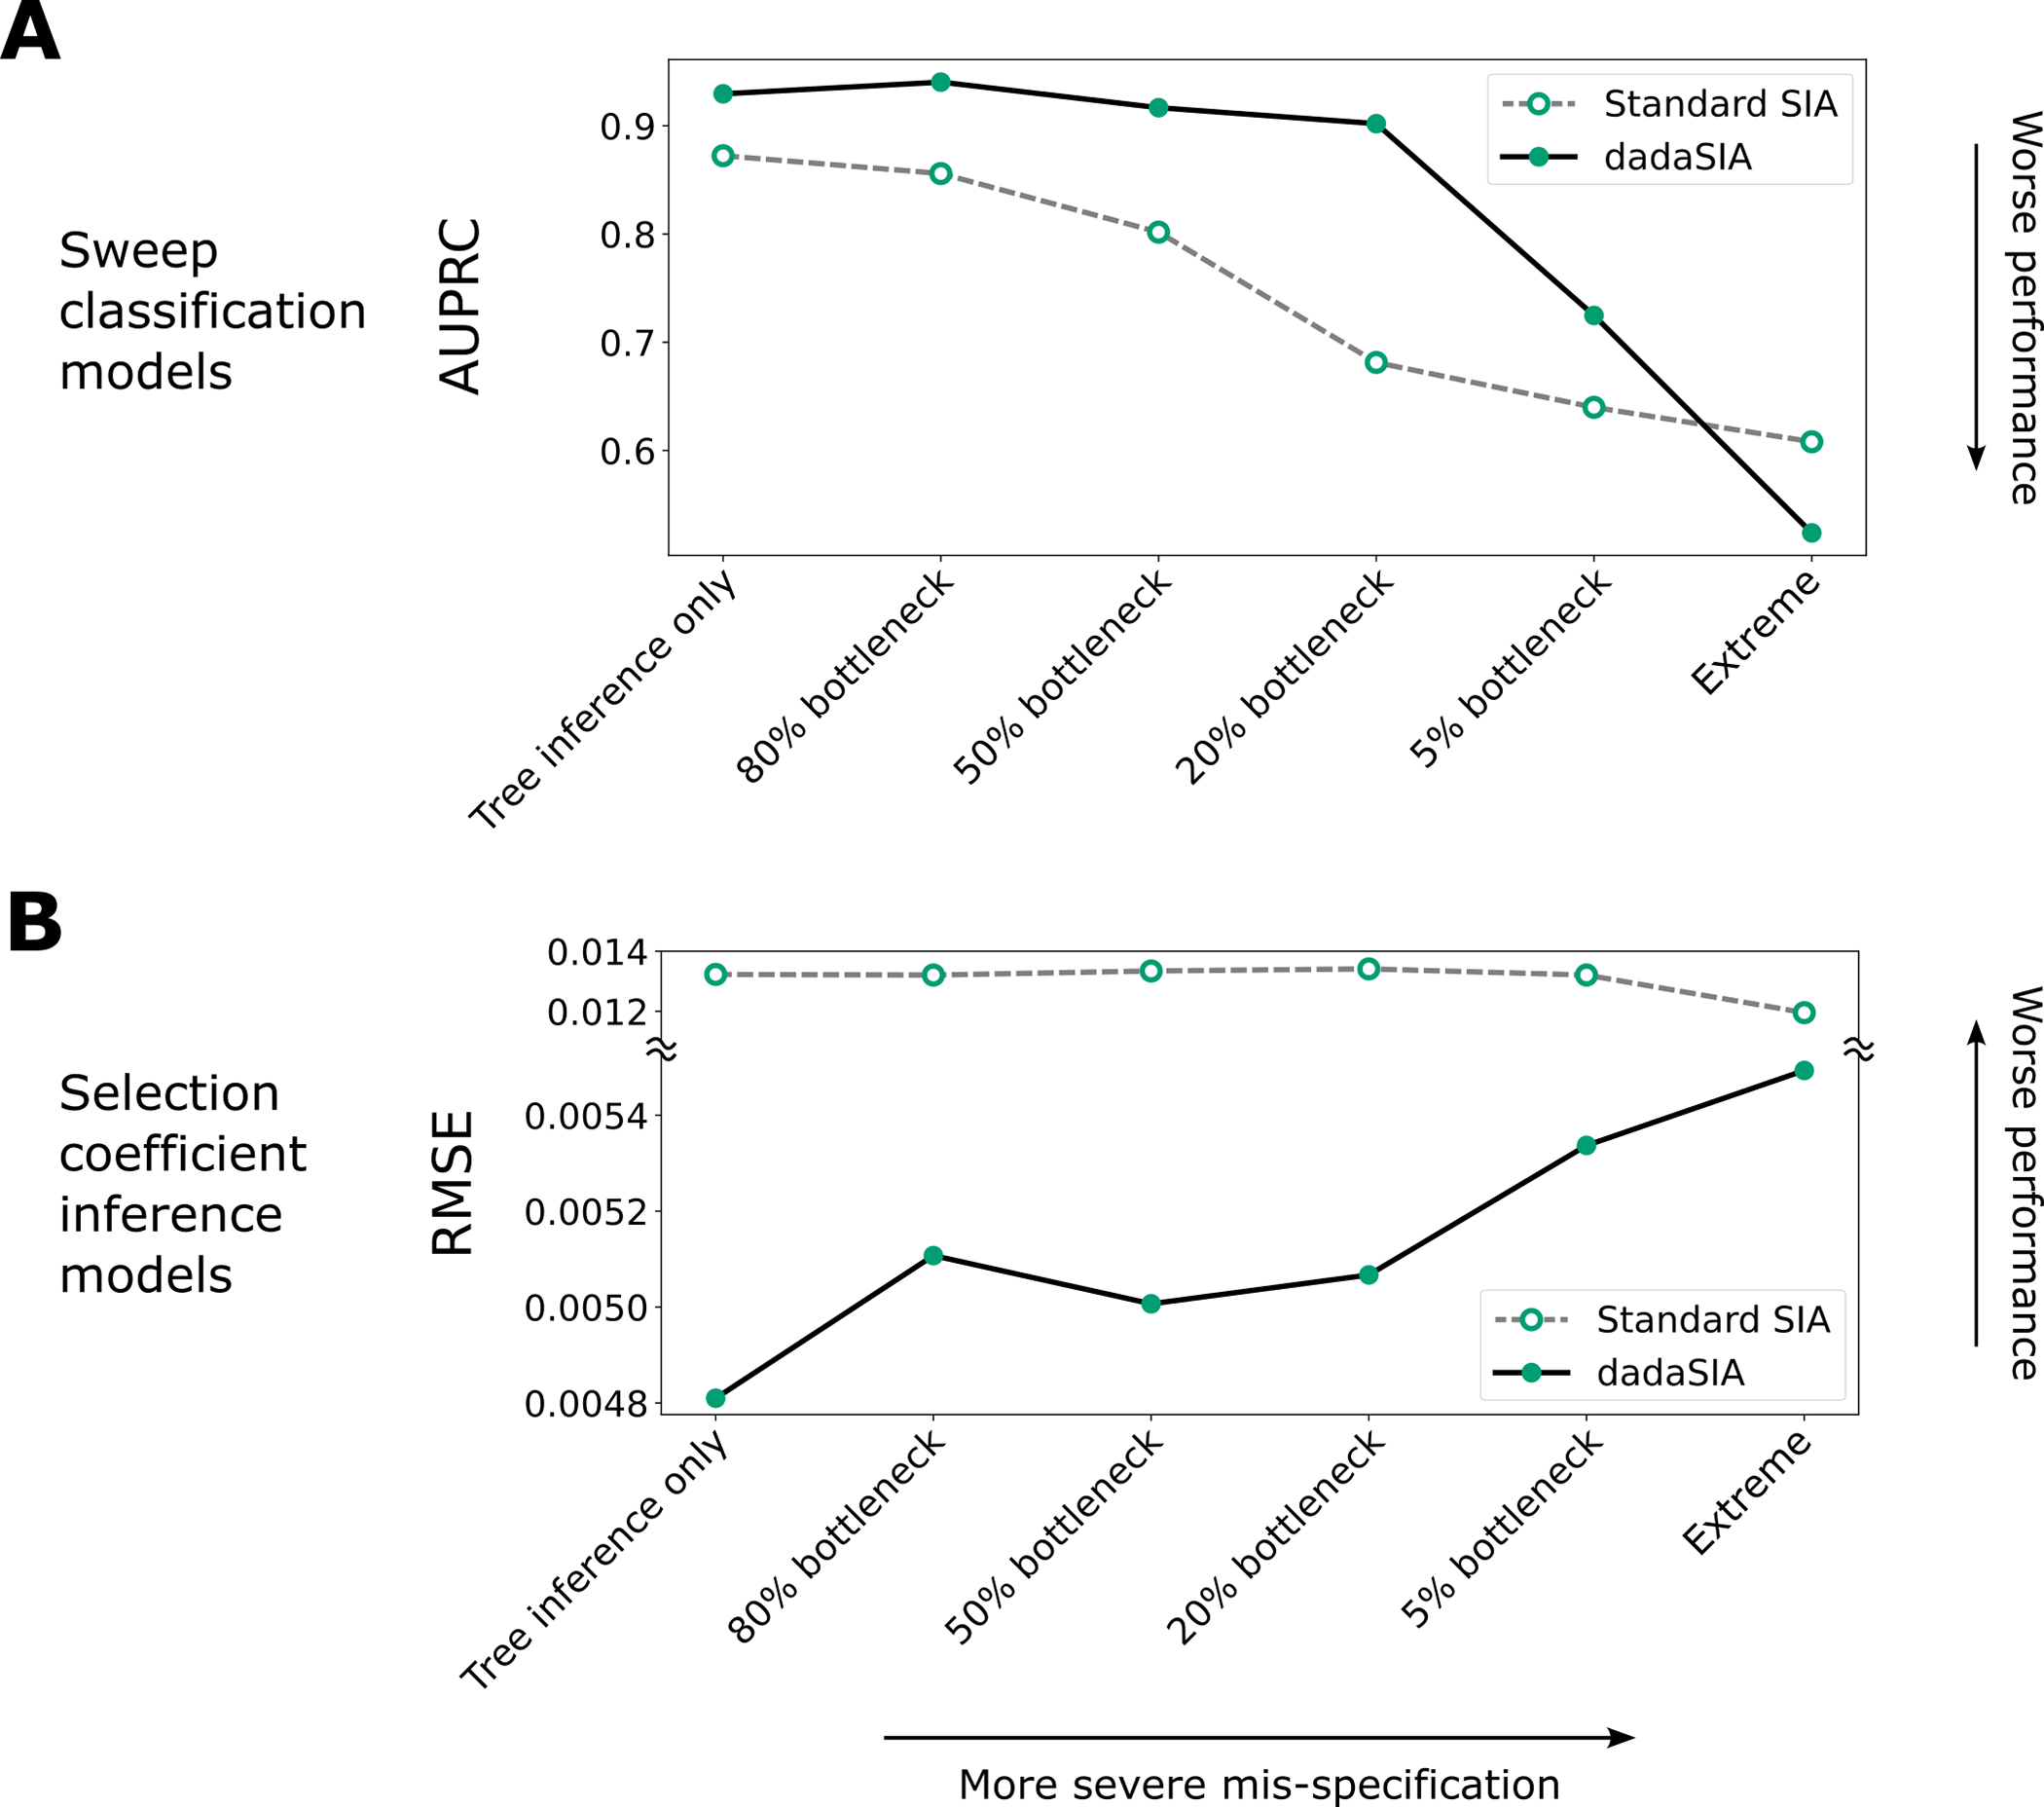
\includegraphics[width=\textwidth]{DA_figs/DA_F5.PNG}
    \caption[Performance of \acf{dadaSIA} model with different degrees of mis-specification.]{\textbf{Performance of \acf{dadaSIA} model with different degrees of mis-specification.} The performance of the model on the sweep classification task is quantified by the \ac{AUPRC} (\textbf{A}). Performance on the selection-coefficient inference task is quantified by \ac{RMSE} (\textbf{B}). In the “tree inference only” case, there is no mis-specification other than that caused by error in genealogy inference. In the “extreme” case, mis-specification consists of a 5\% bottleneck, background selection and an 8-fold mis-specification in recombination rate. See Fig. \href{https://journals.plos.org/plosgenetics/article?id=10.1371/journal.pgen.1011032\#sec018}{S4 online} for illustrations of the different bottlenecks and \nameref{DA-methods} for details.}
    \label{fig:DA-F5}
\end{figure}

Does domain adaptation compromise performance at the opposite extreme, where there is little or no simulation mis-specification? To address this question, we tested the standard and domain-adaptive ReLERNN models in a setting without any simulation mis-specification. We focused here on ReLERNN, which directly uses raw genotypic data, as opposed to SIA, which always has some mis-specification due to genealogy inference error. We observed that the standard and domain-adaptive ReLERNN models performed nearly identically when no mis-specification was present, with only minor decreases in performance (Fig. \href{https://journals.plos.org/plosgenetics/article?id=10.1371/journal.pgen.1011032#sec018}{S7 online}). Thus, there is perhaps some cost in using domain adaptation when it is not needed, but, at least in our case, that cost appears to be slight.

\subsection{Application of domain-adaptive \ac{SIA} to real data}
In applications to real data, the true selection coefficient is not known, so it is impossible to perform a definitive comparison of methods. Nevertheless, it can be informative to evaluate the degree to which alternative methods are concordant, especially with consideration of their relative performance in simulation studies.

Toward this end, we re-applied our \acf{dadaSIA} model to several loci in the human genome that we previously analyzed with \ac{SIA} (\cite{hejase_deep-learning_2022}), using whole-genome sequence data from the 1000 Genomes CEU population (\cite{auton_global_2015}). For the target domain, we sampled genealogies from genome-wide \acp{ARG} inferred from the individual sequences (see \nameref{DA-methods}). The putative causal loci analyzed included \acp{SNP} at the \textit{LCT} gene (\cite{bersaglieri_genetic_2004}), one of the best-studied cases of selective sweeps in the human genome; at the disease-associated genes \textit{TCF7L2} (\cite{lyssenko_mechanisms_2007}), \textit{ANKK1} (\cite{spellicy_variant_2014}) and \textit{FTO} (\cite{frayling_common_2007}); at the pigmentation genes \textit{KITLG} (\cite{sulem_genetic_2007}), \textit{ASIP} (\cite{eriksson_web-based_2010}), \textit{TYR} (\cite{sulem_genetic_2007,eriksson_web-based_2010}), \textit{OCA2} (\cite{han_genome-wide_2008,sturm_single_2008}), \textit{TYRP1} (\cite{kenny_melanesian_2012}) and \textit{TTC3} (\cite{liu_digital_2010}), which were also analyzed by \cite{stern_approximate_2019}; and at the genes \textit{MC1R} (\cite{sulem_genetic_2007,han_genome-wide_2008}) and \textit{ABCC11} (\cite{yoshiura_snp_2006}), where \ac{SIA} reported novel signals of selection.

We found that \ac{dadaSIA} generally made similar predictions to \ac{SIA} at these \acp{SNP}, but there were some notable differences. The seven loci predicted by SIA to be sweeps were also predicted by dadaSIA to be sweeps (Table \ref{tab:DA-T1}), although \ac{dadaSIA} always reported higher confidence in these predictions (with probability of neutrality, $P_{\mathrm{neu}}<10^{-2}$ in all cases) than did \ac{SIA} ($P_{\mathrm{neu}}$ up to 0.384 for \textit{TYR}). The five loci predicted by \ac{SIA} not to be sweeps were also predicted by \ac{dadaSIA} not to be sweeps ($P_{\mathrm{neu}}>0.5$). At \textit{LCT}, the strongest sweep considered, the selection coefficient ($s$) estimated by \ac{dadaSIA} remained very close to \ac{SIA}’s previous estimate of $s = 0.01$ and also close to several prior estimates (\cite{bersaglieri_genetic_2004,mathieson_estimating_2020,mathieson_fads1_2018}). In all other cases, the estimate from \ac{SIA} was somewhat revised by \ac{dadaSIA}, generally by factors of about 2-3. Importantly, in all cases, the estimates from \ac{dadaSIA} remained much closer to those from \ac{SIA} than to estimates by other methods (Table \ref{tab:DA-T1}). Together, these observations suggest that the addition of domain adaptation does not radically alter \ac{SIA}’s predictions for real data but may in some cases improve them (see \nameref{DA-discussion}).

\begin{sidewaystable}
    \centering
    \caption{Selection coefficients in the European population estimated by domain-adaptive \ac{SIA} compared to previous estimates.}
    \vspace{5mm}
    \begin{tabular}{l | l | m{5cm} l m{8cm}}
    \hline
    % https://tex.stackexchange.com/questions/269547/rowcolor-for-a-multirow
       & & \multicolumn{3}{c}{\textbf{Estimates of selection coefficient}} \\ \cline{3-5}
      \rowcolor{white} \multirow{-2}{*}{\textbf{Gene}} & \multirow{-2}{*}{\textbf{\ac{SNP}}} & \textbf{Domain-adaptive SIA} & \textbf{SIA}* & \textbf{Previous estimates} \\ \hline
      \textit{KITLG} & rs12821256 & 0.0035 & 0.0019 & 0.0161 (\cite{stern_approximate_2019}) \\
      \textit{ASIP} & rs619865 & 0.0057 & 0.0019 & 0.0974 (\cite{stern_approximate_2019}) \\
      \textit{TYR} & rs1393350 & 0.0028 & 0.0011 & 0.0112 (\cite{stern_approximate_2019}) \\
      \textit{OCA2} & rs12913832 & 0.0093 & 0.0056 & 0.002 (\cite{stern_approximate_2019}); 0.036 (\cite{wilde_direct_2014}) \\
      \textit{MC1R} & rs1805007 & 0.0027 & 0.0037 & No selection (\cite{harding_evidence_2000}) \\
      \textit{ABCC11} & rs17822931 & 0.0020 & 0.00035 & $\approx$ 0.01 in East Asian (\cite{ohashi_impact_2011}) \\
      \textit{LCT} & rs4988235 & 0.0097 & 0.010 & $\approx$ 0.01 (\cite{bersaglieri_genetic_2004,mathieson_fads1_2018,mathieson_estimating_2020}) \\
      \textit{TYRP1} & rs13289810 & $P_{\mathrm{neu}}>0.5$ & $P_{\mathrm{neu}}>0.5$ & No selection (\cite{stern_approximate_2019}) \\
      \textit{TTC3} & rs1003719 & $P_{\mathrm{neu}}>0.5$ & $P_{\mathrm{neu}}>0.5$ & No selection (\cite{stern_approximate_2019}) \\
      \textit{TCF7L2} & rs7903146 & $P_{\mathrm{neu}}>0.5$ & $P_{\mathrm{neu}}>0.5$ & N/A \\
      \textit{ANKK1} & rs1800497 & $P_{\mathrm{neu}}>0.5$ & $P_{\mathrm{neu}}>0.5$ & N/A \\
      \textit{FTO} & rs9939609 & $P_{\mathrm{neu}}>0.5$ & $P_{\mathrm{neu}}>0.5$ & N/A \\
      \hline
      \rowcolor{white} \multicolumn{5}{p{20cm}}{*The original \ac{SIA} model in \cite{hejase_deep-learning_2022} uses genealogies \textit{inferred} from simulations for training, despite the availability of ground truth genealogies.}
    \end{tabular}
    \label{tab:DA-T1}
\end{sidewaystable}

\section{Discussion} \label{DA-discussion}
Standard approaches to supervised machine learning rest on the assumption that the data they are used to analyze follow essentially the same distribution as the data used for training. In applications in population genetics, the training data are typically generated by simulation, leading to concerns about potential biases from simulation mis-specification when supervised machine-learning methods are used in place of more traditional summary-statistic- or model-based methods (\cite{caldas_inference_2022,korfmann_deep_2023}). In this article, we have shown that techniques from the “domain adaptation” literature can effectively be used to address this problem. In particular, we showed that the addition of \iac{GRL} to two recently developed deep-learning methods for population genetic analysis -- \ac{SIA} and ReLERNN -- led to clear improvements in performance on “real” data that differed in subtle but important ways from the data used to train the models. These improvements were observed both when the demographic models were mis-specified and when background selection was included in the simulations of “real” data but un-modeled in the training data.



\section{Methods} \label{DA-methods}

\section{Supplementary material}
Supporting information is available at \href{https://journals.plos.org/plosgenetics/article?id=10.1371/journal.pgen.1011032#sec018}{\textit{PLoS Genetics} online}. All code used in this study are available at \href{https://github.com/ziyimo/popgen-dom-adapt}{GitHub}. The 1000 Genomes data are available \href{https://www.internationalgenome.org/data}{online}.
